% beamer_template.tex
% 2014-06-18 dmontaner@cipf.es
% Beamer template. Ready to use with pandoc

% For templates see:
% http://deic.uab.es/~iblanes/beamer_gallery/
% For colors see:
% http://deic.uab.es/~iblanes/beamer_gallery/index_by_color.html

%% Latex themes seem to be stored here:
%% /usr/share/texmf/tex/latex/beamer/base/themes

%% tree /usr/share/texmf/tex/latex/beamer/base/themes
%% ├── color
%% │   ├── beamercolortheme...albatross.sty
%% │   ├── beamercolortheme...beaver.sty
%% │   ├── beamercolortheme...beetle.sty
%% │   ├── beamercolortheme...crane.sty
%% │   ├── beamercolortheme...default.sty
%% │   ├── beamercolortheme...dolphin.sty
%% │   ├── beamercolortheme...dove.sty
%% │   ├── beamercolortheme...fly.sty
%% │   ├── beamercolortheme...lily.sty
%% │   ├── beamercolortheme...monarca.sty
%% │   ├── beamercolortheme...orchid.sty
%% │   ├── beamercolortheme...rose.sty
%% │   ├── beamercolortheme...seagull.sty
%% │   ├── beamercolortheme...seahorse.sty
%% │   ├── beamercolortheme...sidebartab.sty
%% │   ├── beamercolortheme...spruce.sty
%% │   ├── beamercolortheme...structure.sty
%% │   ├── beamercolortheme...whale.sty
%% │   └── beamercolortheme...wolverine.sty
%% ├── font
%% │   ├── beamerfonttheme...default.sty
%% │   ├── beamerfonttheme...professionalfonts.sty
%% │   ├── beamerfonttheme...serif.sty
%% │   ├── beamerfonttheme...structurebold.sty
%% │   ├── beamerfonttheme...structureitalicserif.sty
%% │   └── beamerfonttheme...structuresmallcapsserif.sty
%% ├── inner
%% │   ├── beamerinnertheme...circles.sty
%% │   ├── beamerinnertheme...default.sty
%% │   ├── beamerinnertheme...inmargin.sty
%% │   ├── beamerinnertheme...rectangles.sty
%% │   └── beamerinnertheme...rounded.sty
%% ├── outer
%% │   ├── beameroutertheme...default.sty
%% │   ├── beameroutertheme...infolines.sty
%% │   ├── beameroutertheme...miniframes.sty
%% │   ├── beameroutertheme...shadow.sty
%% │   ├── beameroutertheme...sidebar.sty
%% │   ├── beameroutertheme...smoothbars.sty
%% │   ├── beameroutertheme...smoothtree.sty
%% │   ├── beameroutertheme...split.sty
%% │   └── beameroutertheme...tree.sty
%% └── theme
%%     ├── beamertheme...AnnArbor.sty
%%     ├── beamertheme...Antibes.sty
%%     ├── beamertheme...Bergen.sty
%%     ├── beamertheme...Berkeley.sty
%%     ├── beamertheme...Berlin.sty
%%     ├── beamertheme...Boadilla.sty
%%     ├── beamertheme...boxes.sty
%%     ├── beamertheme...CambridgeUS.sty
%%     ├── beamertheme...Copenhagen.sty
%%     ├── beamertheme...Darmstadt.sty
%%     ├── beamertheme...default.sty
%%     ├── beamertheme...Dresden.sty
%%     ├── beamertheme...EastLansing.sty
%%     ├── beamertheme...Frankfurt.sty
%%     ├── beamertheme...Goettingen.sty
%%     ├── beamertheme...Hannover.sty
%%     ├── beamertheme...Ilmenau.sty
%%     ├── beamertheme...JuanLesPins.sty
%%     ├── beamertheme...Luebeck.sty
%%     ├── beamertheme...Madrid.sty
%%     ├── beamertheme...Malmoe.sty
%%     ├── beamertheme...Marburg.sty
%%     ├── beamertheme...Montpellier.sty
%%     ├── beamertheme...PaloAlto.sty
%%     ├── beamertheme...Pittsburgh.sty
%%     ├── beamertheme...Rochester.sty
%%     ├── beamertheme...Singapore.sty
%%     ├── beamertheme...Szeged.sty
%%     ├── beamertheme...Warsaw.sty
%%     └── compatibility
%%         ├── beamertheme...bars.sty
%%         ├── beamertheme...classic.sty
%%         ├── beamertheme...compatibility.sty
%%         ├── beamertheme...lined.sty
%%         ├── beamertheme...plain.sty
%%         ├── beamertheme...shadow.sty
%%         ├── beamertheme...sidebar.sty
%%         ├── beamertheme...split.sty
%%         └── beamertheme...tree.sty


%% Inner Themes
%% =============================================================================

%% An inner theme installs templates that dictate how the following elements 
%% are typeset:
%% - Title and part pages.
%% - Itemize environments.
%% - Enumerate environments.
%% - Description environments.
%% - Block environments.
%% - Theorem and proof environments.
%% - Figures and tables.
%% - Footnotes.
%% - Bibliography entries.

%% Outer Themes
%% =============================================================================
%% An outer theme dictates the overall layout of frames. 
%% It specifies where any navigational elements should go 
%% and what they should look like. 

%% An outer theme specifies how the following elements are rendered:
%% - The head- and footline.
%% - The sidebars.
%% - The logo.
%% - The frame title.

%%%%%%%%%%%%%%%%%%%%%%%%%%%%%%%%%%%%%%%%%%%%%%%%%%%%%%%%%%%%%%%%%%%%%%%%%%%%%%%%
%%% TEMPLATE
%%%%%%%%%%%%%%%%%%%%%%%%%%%%%%%%%%%%%%%%%%%%%%%%%%%%%%%%%%%%%%%%%%%%%%%%%%%%%%%%

%% Document
\documentclass{beamer}
\usepackage[utf8]{inputenc}
\usepackage[T1]{fontenc} % Spanish characters
\usepackage{lmodern}     % Use always with T1. Otherwise the letter looks weird.
%\usepackage{graphicx}   % ??? SEE WHY IS NOT ON

%% TABLES
\usepackage{longtable,booktabs}        % the package is needed in Pandoc
\usepackage{caption}
\makeatletter                          % These lines are needed 
\def\fnum@table{\tablename~\thetable}  % to make table captions 
\makeatother                           % work with longtable.


%%%%%%%%%%%%%%%%%%%%%%%%%%%%%%%%%%%%%%%%%%%%%%%%%%%%%%%%%%%%%%%%%%%%%%%%%%%%%%%%
%%% PARAMETERS (has to be here: after the utf8 encoding)
%%%%%%%%%%%%%%%%%%%%%%%%%%%%%%%%%%%%%%%%%%%%%%%%%%%%%%%%%%%%%%%%%%%%%%%%%%%%%%%%

%% \def \titulolargo {This is my LONG title} % long title:  this will go to the FIRST slide.
%% \def \titulocorto {short title}           % short title: this will go to the FOOTER of the slides.
%% \def \subtitulo {my subtitle}
%% \def \autorlargo {David Montaner} % long author:  this will go to the FIRST slide.
%% \def \autorcorto {D. Montaner}    % short author: this will go to the FOOTER of the slides.
%% \def \fecha {mifecha 2014-06-18}


%% to be used as a pandoc template
\def \titulolargo {NGS Data Analysis Course}         % long title:  this will go to the FIRST slide.
\def \titulocorto {NGS Data Analysis Course}  % short title: this will go to the FOOTER of the slides.
\def \subtitulo {RNA-Seq Analysis}
\def \autorlargo {Marta Bleda, Javier Lopez, Ignacio Medina, David Montaner}         % long author:  this will go to the FIRST slide.
\def \autorcorto {RNA-Seq Analysis}    % short author: this will go to the FOOTER of the slides.
\def \fecha {2015-02-23}
\def \pagina {http://www.ngscourse.org}


%% My Beamer Combinations %%%%%%%%%%%%%%%%%%%%%%%%%%%%%%%%%%%%%%%%%%%%%%%%%%%%%%

%% % Orange
%% \useinnertheme[shadow]{rounded}
%% \usecolortheme{crane}
%% \useoutertheme{shadow}  % INCLUDES THE FOOTER

% Light blue
\useinnertheme[shadow]{rounded}
\usecolortheme{seahorse}
\useoutertheme{shadow}  % INCLUDES THE FOOTER

% Strong blue
%% \useinnertheme[shadow]{rounded}
%% \usecolortheme{whale}
%% \useoutertheme{shadow}  % INCLUDES THE FOOTER

%%%%%%%%%%%%%%%%%%%%%%%%%%%%%%%%%%%%%%%%%%%%%%%%%%%%%%%%%%%%%%%%%%%%%%%%%%%%%%%%


%% beamer theme INNER
%\useinnertheme{default}
%\useinnertheme{rectangles} %squared bullets
%\useinnertheme{circles}    %circular bullets
%\useinnertheme{rounded}         % bullets as balls, round borders                               FAVORITE ; use with seahorse and whale
%\useinnertheme[shadow]{rounded} % bullets as balls, round borders and shadow under the boxes    FAVORITE ; do not use with seahorse or whale


%% beamer theme OUTER
%\useoutertheme{default}
%\useoutertheme{infolines} % with slide number but I do not like it. It has also sections. The title is short.
%\useoutertheme{split}  
%\useoutertheme{shadow}    % INCLUDES THE FOOTER


%% beamer COLOR
%% SEE http://deic.uab.es/~iblanes/beamer_gallery/index_by_color.html

%\usecolortheme{whale}     % dark blue             FAVORITE
%\usecolortheme{seahorse}  % light blue            FAVORITE
%\usecolortheme{crane}     % orange and squared    FAVORITE

%\usecolortheme{default}
%\usecolortheme{orchid}    % white background
%\usecolortheme{dove}      % white background and black titles. Not nice boxes
%\usecolortheme{rose}      % white background; blocks are OK in blue
%\usecolortheme{wolverine} % orange yellow; no squares
%\usecolortheme{fly}       % gray Background
%\usecolortheme{beetle}    % gray Background and blue titles. Not very interesting.


%% beamer FONT
%\usefonttheme{default}      % sans serif font f
\usefonttheme{structurebold} % nice font (I do not know which is it)


% beamer EXTRA options (set them after the theme)
\setbeamertemplate{frametitle}[default][center] % centering titles
\setbeamertemplate{navigation symbols}{}        % suppresses all navigation symbols

\setbeamertemplate{caption}{\insertcaption}     % suppresses the 'Figure' tagging in images
\setbeamertemplate{caption label separator}{}


%%%%%%%%%%%%%%%%%%%%%%%%%%%%%%%%%%%%%%%%%%%%%%%%%%%%%%%%%%%%%%%%%%%%%%%%%%%%%%%%

%%% GENERAL SETTINGS

%% Color links
\definecolor{links}{HTML}{2A1B81}                  % color for links SEE IF THEY WORK WITH ALL THEMES: 'whale', 'seahorse' and 'crane'.
\hypersetup{colorlinks,linkcolor=,urlcolor=links}

%% Color verbatim
\makeatletter 
\renewcommand\verbatim@font{\normalfont\ttfamily\color{violet}}  % not too bad for all my theme combinations.
%\renewcommand\verbatim@font{\normalfont\ttfamily\color{orange}}
%\renewcommand\verbatim@font{\normalfont\ttfamily\color{blue}}
%\renewcommand\verbatim@font{\normalfont\ttfamily\color{green}}
%\renewcommand\verbatim@font{\normalfont\ttfamily\color{gray}}
%\renewcommand\verbatim@font{\normalfont\ttfamily\color{red}}
%\renewcommand\verbatim@font{\normalfont\ttfamily\color{pink}}
\makeatother

%% % Scale images as in the pandoc template
%% % WORKS but if used 'scale' DOES NOT WORK
%% \usepackage{graphicx}
%% \makeatletter
%% \def \maxwidth  {\ifdim \Gin@nat@width  > \linewidth     \linewidth    \else \Gin@nat@width  \fi}
%% \def \maxheight {\ifdim \Gin@nat@height > \textheight   0.8\textheight \else \Gin@nat@height \fi}
%% \makeatother
%% % Scale images if necessary, so that they will not overflow the page
%% % margins by default, and it is still possible to overwrite the defaults
%% % using explicit options in \includegraphics[width, height, ...]{}
%% \setkeys{Gin}{width=\maxwidth,height=\maxheight,keepaspectratio}

%% Separation between paragraphs
%\setlength{\parskip}{\baselineskip}
%\parskip=1.5ex % ex is a vertical measure

%% Bullet separation from previous paragraph: IMPOSSIBLE
%% see: <http://tex.stackexchange.com/questions/115907/how-do-i-remove-white-space-above-itemize-command-in-beamer-using-enumitem>
%% It's not a good idea to use the enumitem package with beamer since beamer has its own ways of dealing with the standard list-like environment
%\usepackage{enumitem}
%\setlist[itemize]{noitemsep, topsep=0pt, partopsep=0pt}



%%%%%%%%%%%%%%%%%%%%%%%%%%%%%%%%%%%%%%%%%%%%%%%%%%%%%%%%%%%%%%%%%%%%%%%%%%%%%%%%
%% TITLE (depends on definde parameters)
%%%%%%%%%%%%%%%%%%%%%%%%%%%%%%%%%%%%%%%%%%%%%%%%%%%%%%%%%%%%%%%%%%%%%%%%%%%%%%%%
\title[{\makebox[.45\paperwidth]{\titulocorto \hfill \insertframenumber/\inserttotalframenumber}}]{\titulolargo}
\subtitle{{\color{gray}\subtitulo}}  %% GREY is nice for the 'whale', 'seahorse' and the 'crane' color themes
%\subtitle{\subtitulo}

\author[\autorcorto]{\autorlargo}

\date{\fecha \newline \newline \url{\pagina}}


%%%%%%%%%%%%%%%%%%%%%%%%%%%%%%%%%%%%%%%%%%%%%%%%%%%%%%%%%%%%%%%%%%%%%%%%%%%%%%%%
%% DOCUMENT %%%%%%%%%%%%%%%%%%%%%%%%%%%%%%%%%%%%%%%%%%%%%%%%%%%%%%%%%%%%%%%%%%%%
%%%%%%%%%%%%%%%%%%%%%%%%%%%%%%%%%%%%%%%%%%%%%%%%%%%%%%%%%%%%%%%%%%%%%%%%%%%%%%%%
\begin{document}

%% title frame
\begin{frame}
  \maketitle
\end{frame}

\begin{frame}{NGS pipeline}

\begin{figure}[htbp]
\centering
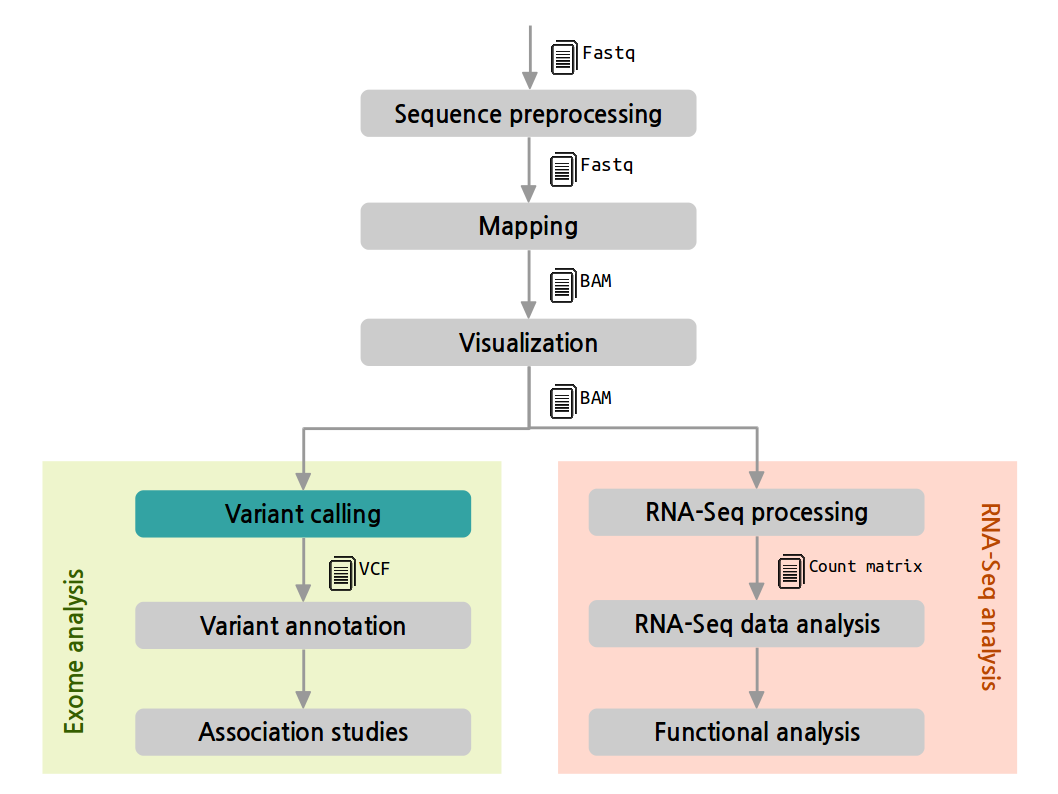
\includegraphics[width=\textwidth,height=0.8\textheight,keepaspectratio]{images/ngs_pipeline.png}

\end{figure}

\end{frame}

\begin{frame}{Experiment considerations}

\begin{itemize}
\itemsep1pt\parskip0pt\parsep0pt
\item
  Reference genome

  \begin{itemize}
  \itemsep1pt\parskip0pt\parsep0pt
  \item
    Yes: map against it
  \item
    No: try to assemble transcripts an then map
  \end{itemize}
\item
  Reference transcriptome

  \begin{itemize}
  \itemsep1pt\parskip0pt\parsep0pt
  \item
    Yes: estimate known transcripts abundance \& discover new
    transcripts
  \item
    No: find expressed regions \& their transcript combination
  \end{itemize}
\end{itemize}

\end{frame}

\begin{frame}{Gene transcript length dependence}

Counts are proportional to \ldots{}

\begin{itemize}
\itemsep1pt\parskip0pt\parsep0pt
\item
  the mRNA expression level
\item
  the \emph{transcript length}
\end{itemize}

\begin{figure}[htbp]
\centering
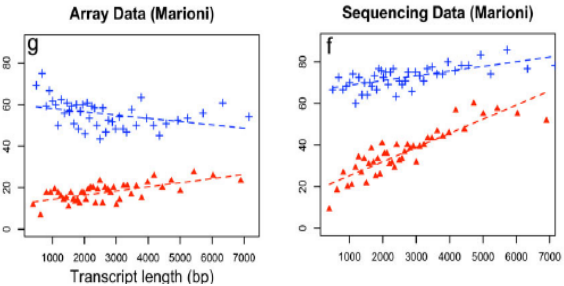
\includegraphics[width=\textwidth,height=0.8\textheight,keepaspectratio]{images/gene_length_dependence.png}

\end{figure}

\end{frame}

\begin{frame}{Gene transcript length dependence}

\begin{figure}[htbp]
\centering
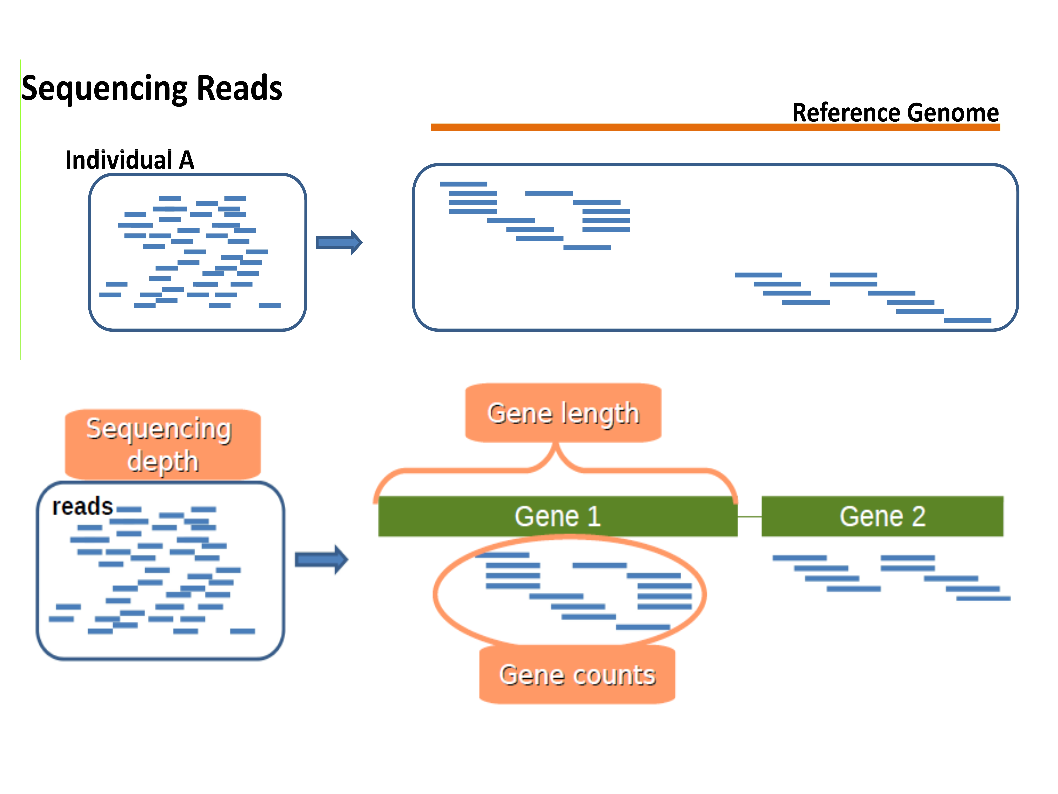
\includegraphics[width=\textwidth,height=0.8\textheight,keepaspectratio]{images/gene_length.png}

\end{figure}

\end{frame}

\begin{frame}{Library size dependence}

More reads in the library -\textgreater{} more reads per transcript

Library size matters.

Correction is needed for some analysis:

\begin{itemize}
\itemsep1pt\parskip0pt\parsep0pt
\item
  Descriptive statistics: PCA, clustering, \ldots{}
\end{itemize}

May not be so important for other analyses:

\begin{itemize}
\itemsep1pt\parskip0pt\parsep0pt
\item
  Differential expression at gene level \ldots{}
\end{itemize}

\end{frame}

\begin{frame}{Count Normalization}

\begin{itemize}
\itemsep1pt\parskip0pt\parsep0pt
\item
  Transcript length: within library
\item
  Library size: between libraries
\item
  Many other biases \ldots{}

  \begin{itemize}
  \itemsep1pt\parskip0pt\parsep0pt
  \item
    Differences on the read count distribution among samples.
  \item
    GC content of the gene affects the detection of that gene (Illumina)
  \item
    sequence-specific bias is introduced during the library preparation
  \end{itemize}
\end{itemize}

\end{frame}

\begin{frame}{RPKM}

\textbf{RPKM}: Reads Per Kilobase of the transcript per Million mapped
reads

\[ RPKM = 10^9 \frac{C}{N L} \]

\begin{itemize}
\itemsep1pt\parskip0pt\parsep0pt
\item
  \textbf{C}: number of reads mapped to the exons of the gene.
\item
  \textbf{N}: total number of mappable reads in the experiment.
\item
  \textbf{L}: total length of the exons of the gene.
\end{itemize}

Fragments Per Kilobase of exon per Million fragments mapped (FPKM)

\end{frame}

\begin{frame}{Many other count corrections}

\begin{itemize}
\itemsep1pt\parskip0pt\parsep0pt
\item
  RPKM (Mortazavi et al., 2008)
\item
  TC: Gene counts are divided by the sequencing depth associated to that
  sample and multiplied by the average of the total counts across all
  the samples. Gene counts are divided by the gene length (kb) times the
  total number of millions of mapped reads.
\item
  Upper-quartile (Bullard et al., 2010): Gene counts are divided by the
  upper quartile of counts for genes with at least one read.
\item
  Median (Bullard et al., 2010): Gene counts are divided by the median
  of counts for genes with at least one read.
\item
  Quantile (Irizarry et al., 2003): This method matches the gene count
  distributions across samples.
\item
  edgeR (Robinson et al., 2009): overdispersed Poisson model.
  Bioconductor package
\end{itemize}

\end{frame}

\begin{frame}{Many other count corrections}

\begin{itemize}
\itemsep1pt\parskip0pt\parsep0pt
\item
  TMM (Robinson \& Oshlack, 2010): Trimmed Mean of M-values. Based on
  the hypothesis that most of the genes are not DE. A sample is taken as
  the reference. For each sample, the scaling factor is the weighted
  mean of log ratios between this sample and the reference after
  removing the most expressed genes and those with the largest log
  ratios. Gene counts are divided by this factor re-scaled by the mean
  of the normalized library sizes.
\item
  DESeq (Anders \& Huber, 2010): Based on the hypothesis that most of
  the genes are not DE.
\item
  The scaling factor for a given sample is the median of the ratio, for
  each gene, of its counts over its geometric mean across all the
  samples. Gene counts are divided by this scaling factor.
\item
  FPKM (Trapnell et al., 2010): implemented in Cufflinks, similar to
  RPKM .
\end{itemize}

\end{frame}

\begin{frame}{Software}

\begin{itemize}
\item
  TopHat / Bowtie: alignment
\item
  Cufflinks:

  \begin{itemize}
  \itemsep1pt\parskip0pt\parsep0pt
  \item
    assembly
  \item
    compare with the known transcripts
  \end{itemize}
\item
  Cuffdiff: differential expression

  \begin{itemize}
  \itemsep1pt\parskip0pt\parsep0pt
  \item
    estimate fragment length distribution
  \item
    calculate transcript abundances FPKM
  \item
    sequence bias correction
  \end{itemize}
\item
  CummeRbund:

  \begin{itemize}
  \itemsep1pt\parskip0pt\parsep0pt
  \item
    an R package to handle results
  \end{itemize}
\end{itemize}

\end{frame}

\begin{frame}{Software}

\begin{figure}[htbp]
\centering
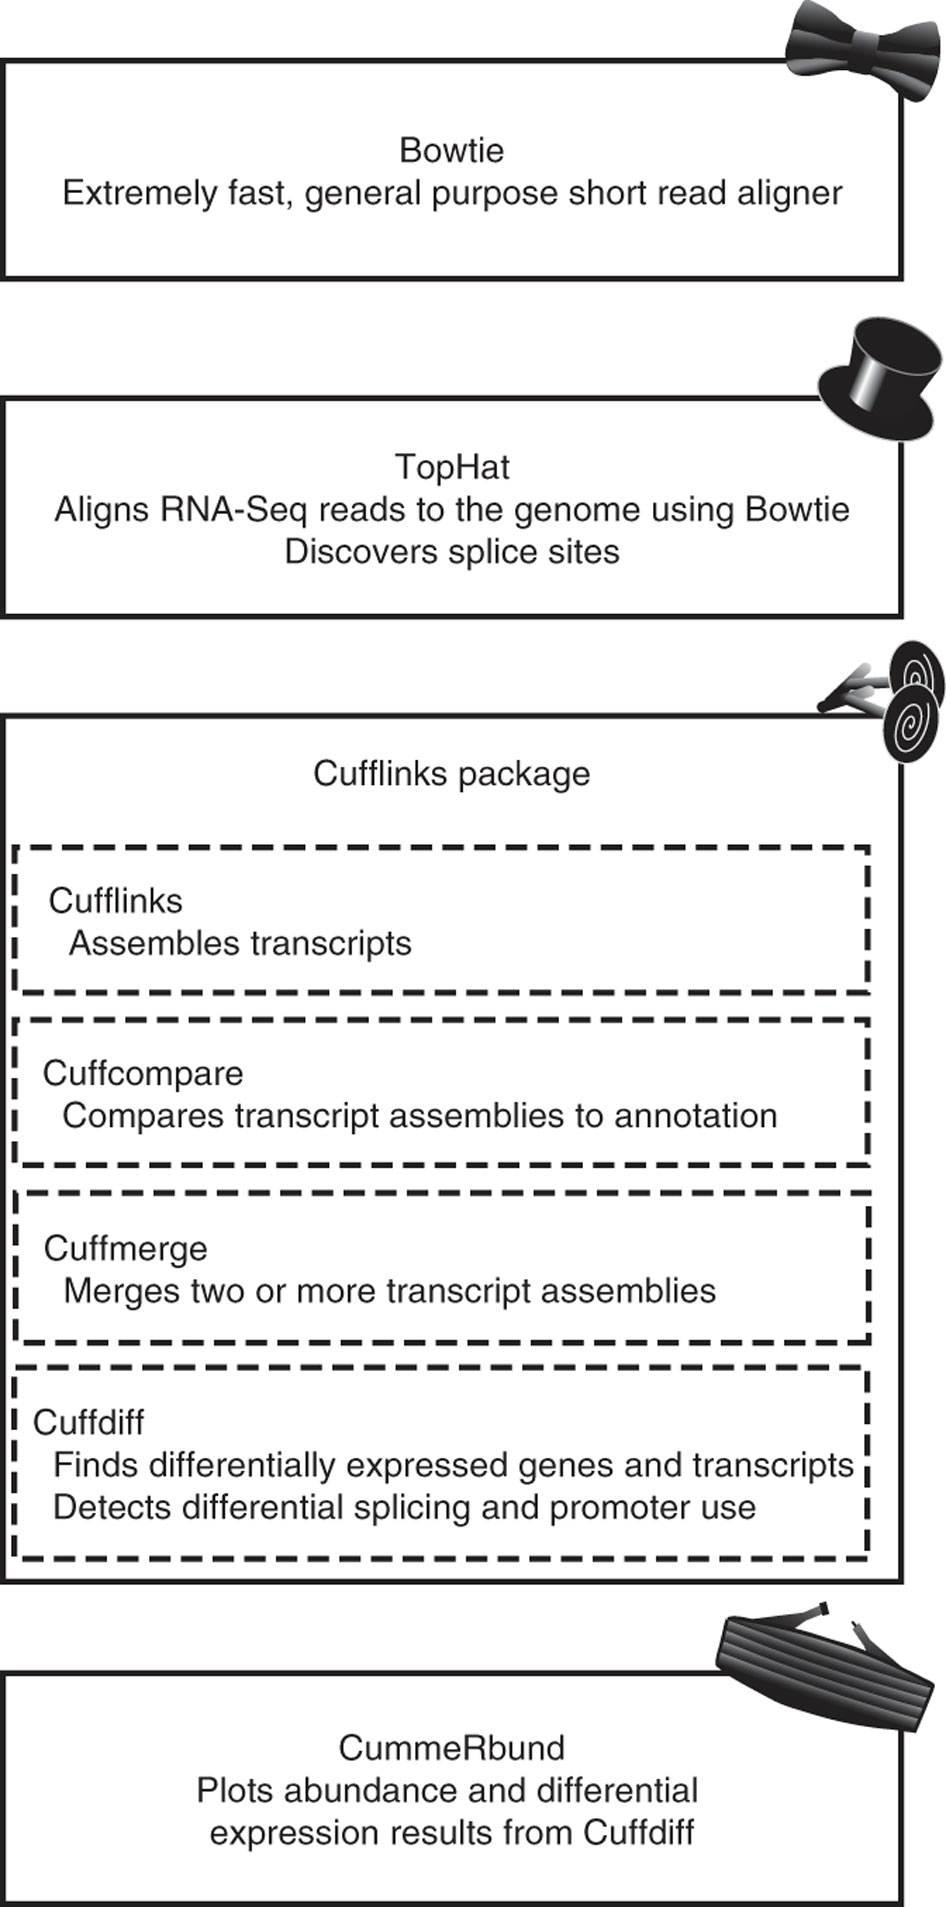
\includegraphics[width=\textwidth,height=0.8\textheight,keepaspectratio]{images/cufflinks_pipeline.png}

\end{figure}

\end{frame}

%% %%%%%%%%%%%%%%%%%%%%%%%%%%%%%%%%%%%%%%%%%%%%%%%%%%%%%%%%%%%%

%% \begin{frame}
%%   \frametitle{Titulo}
%%   \framesubtitle{SubTitulo}
  
%%   \begin{itemize}
%%   \item uno
%%   \item dos
%%   \end{itemize}  

%%   \url{http://www.dmontaner.com/}

%%   \href{http://www.dmontaner.com/}{un link}

%%   \begin{enumerate}
%%   \item uno número
%%   \item dos número
%%   \end{enumerate}  

%% \end{frame}

%% %%%%%%%%%%%%%%%%%%%%%%%%%%%%%%%%%%%%%%%%%%%%%%%%%%%%%%%%%%%%

%% \begin{frame}[fragile]
%%   \frametitle{Verbatim}
  
%%   Este es un texto en \texttt{verbatim}
  
%%   \begin{verbatim}

%%     ver si no sera mejor ponerle un background
    
%%     texto o codigo tal cual 
%%     texto o codigo  tal cual hasta con espacios
    
%%   \end{verbatim}
  
%% \end{frame}

%% %%%%%%%%%%%%%%%%%%%%%%%%%%%%%%%%%%%%%%%%%%%%%%%%%%%%%%%%%%%%

%% \begin{frame}
%%   \frametitle{Parrafos}

%%   PRIMER PARRAFO: Don Juan Carlos, de 76 años, se ha dirigido a la nación a través 
%%   de la televisión pública para explicar los motivos de su renuncia: 
  
%%   AQUI EMPIEZA EL SEGUNDO PARRAFO: "Hoy merece pasar a la primera línea una generación 
%%   más joven, con nuevas energías y con una nueva forma de enfrentar la realidad".
  
  
%%   \begin{itemize}
%%   \item uno
%%   \item dos
%%   \end{itemize}  
  
%%   AQUI EMPIEZA EL TERCER PARRAFO: El Rey ha agradecido su ayuda a la Reina durante 
%%   todos estos años; ha dicho que el Príncipe Felipe cuenta con la "madurez, 
%%   la preparación y el compromiso necesarios" para ser el próximo jefe del Estado,
%%   y ha recordado que éste cuenta con "el apoyo de la Princesa Letizia".

%% \end{frame}

%% %%%%%%%%%%%%%%%%%%%%%%%%%%%%%%%%%%%%%%%%%%%%%%%%%%%%%%%%%%%%

%% \begin{frame}
%%   \frametitle{Images: big}
%%   \includegraphics[width=\textwidth,height=0.8\textheight,keepaspectratio]{images/big}
%% \end{frame}

%% \begin{frame}
%%   \frametitle{Images: small}
%%   \includegraphics[width=\textwidth,height=0.8\textheight,keepaspectratio]{images/small}
%% \end{frame}

%% %%%

%% \begin{frame}
%%   \frametitle{Images: big SCALED}
%%   \includegraphics[width=\textwidth,height=0.8\textheight,keepaspectratio]{images/big}
%% \end{frame}

%% \begin{frame}
%%   \frametitle{Images: small SCALED}
%%   \includegraphics[width=\textwidth,height=0.8\textheight,keepaspectratio]{images/small}
%% \end{frame}

%% %%%

%% \begin{frame}
%%   \frametitle{Images: big RE-SCALED}
%%   \includegraphics[scale=0.1]{images/big}
%% \end{frame}

%% %%%%%%%%%%%%%%%%%%%%%%%%%%%%%%%%%%%%%%%%%%%%%%%%%%%%%%%%%%%%

%% \begin{frame}
%%   \frametitle{Bloques}
  
%%   Van los bloques a ver como se organizan.

%%   \begin{block}{Bloque uno}
%%     una cosa aqui dentro
%%   \end{block}


%%   \begin{block}{Otro bloque}
%%     \begin{itemize}
%%     \item uno
%%     \item dos
%%     \end{itemize}  
%%   \end{block}

%%   Con una linea de separacion

%%   \begin{block}{Bloque uno}
%%     otra cosa aqui dentro
%%   \end{block}

%%   Y fuera del utlimo bloque

%% \end{frame}

%% %%%%%%%%%%%%%%%%%%%%%%%%%%%%%%%%%%%%%%%%%%%%%%%%%%%%%%%%%%%%

%% \begin{frame}
%%   \frametitle{Cosita}
  
%%   Que hace esto

%%   ~ 

%%   parece que deja un doble espacio entre parrafos

%%   de todo

%% \end{frame}



%%%%%%%%%%%%%%%%%%%%%%%%%%%%%%%%%%%%%%%%%%%%%%%%%%%%%%%%%%%%%%%%%%%%%%%%%%%%%%%%
%% DOCUMENT END %%%%%%%%%%%%%%%%%%%%%%%%%%%%%%%%%%%%%%%%%%%%%%%%%%%%%%%%%%%%%%%%
\end{document}
